\documentclass{standalone}
\usepackage{tikz}
\usetikzlibrary{patterns, positioning}
\usepackage[sfdefault]{ClearSans} %% option 'sfdefault' activates Clear Sans as the default text font
\usepackage[T1]{fontenc}

\begin{document}
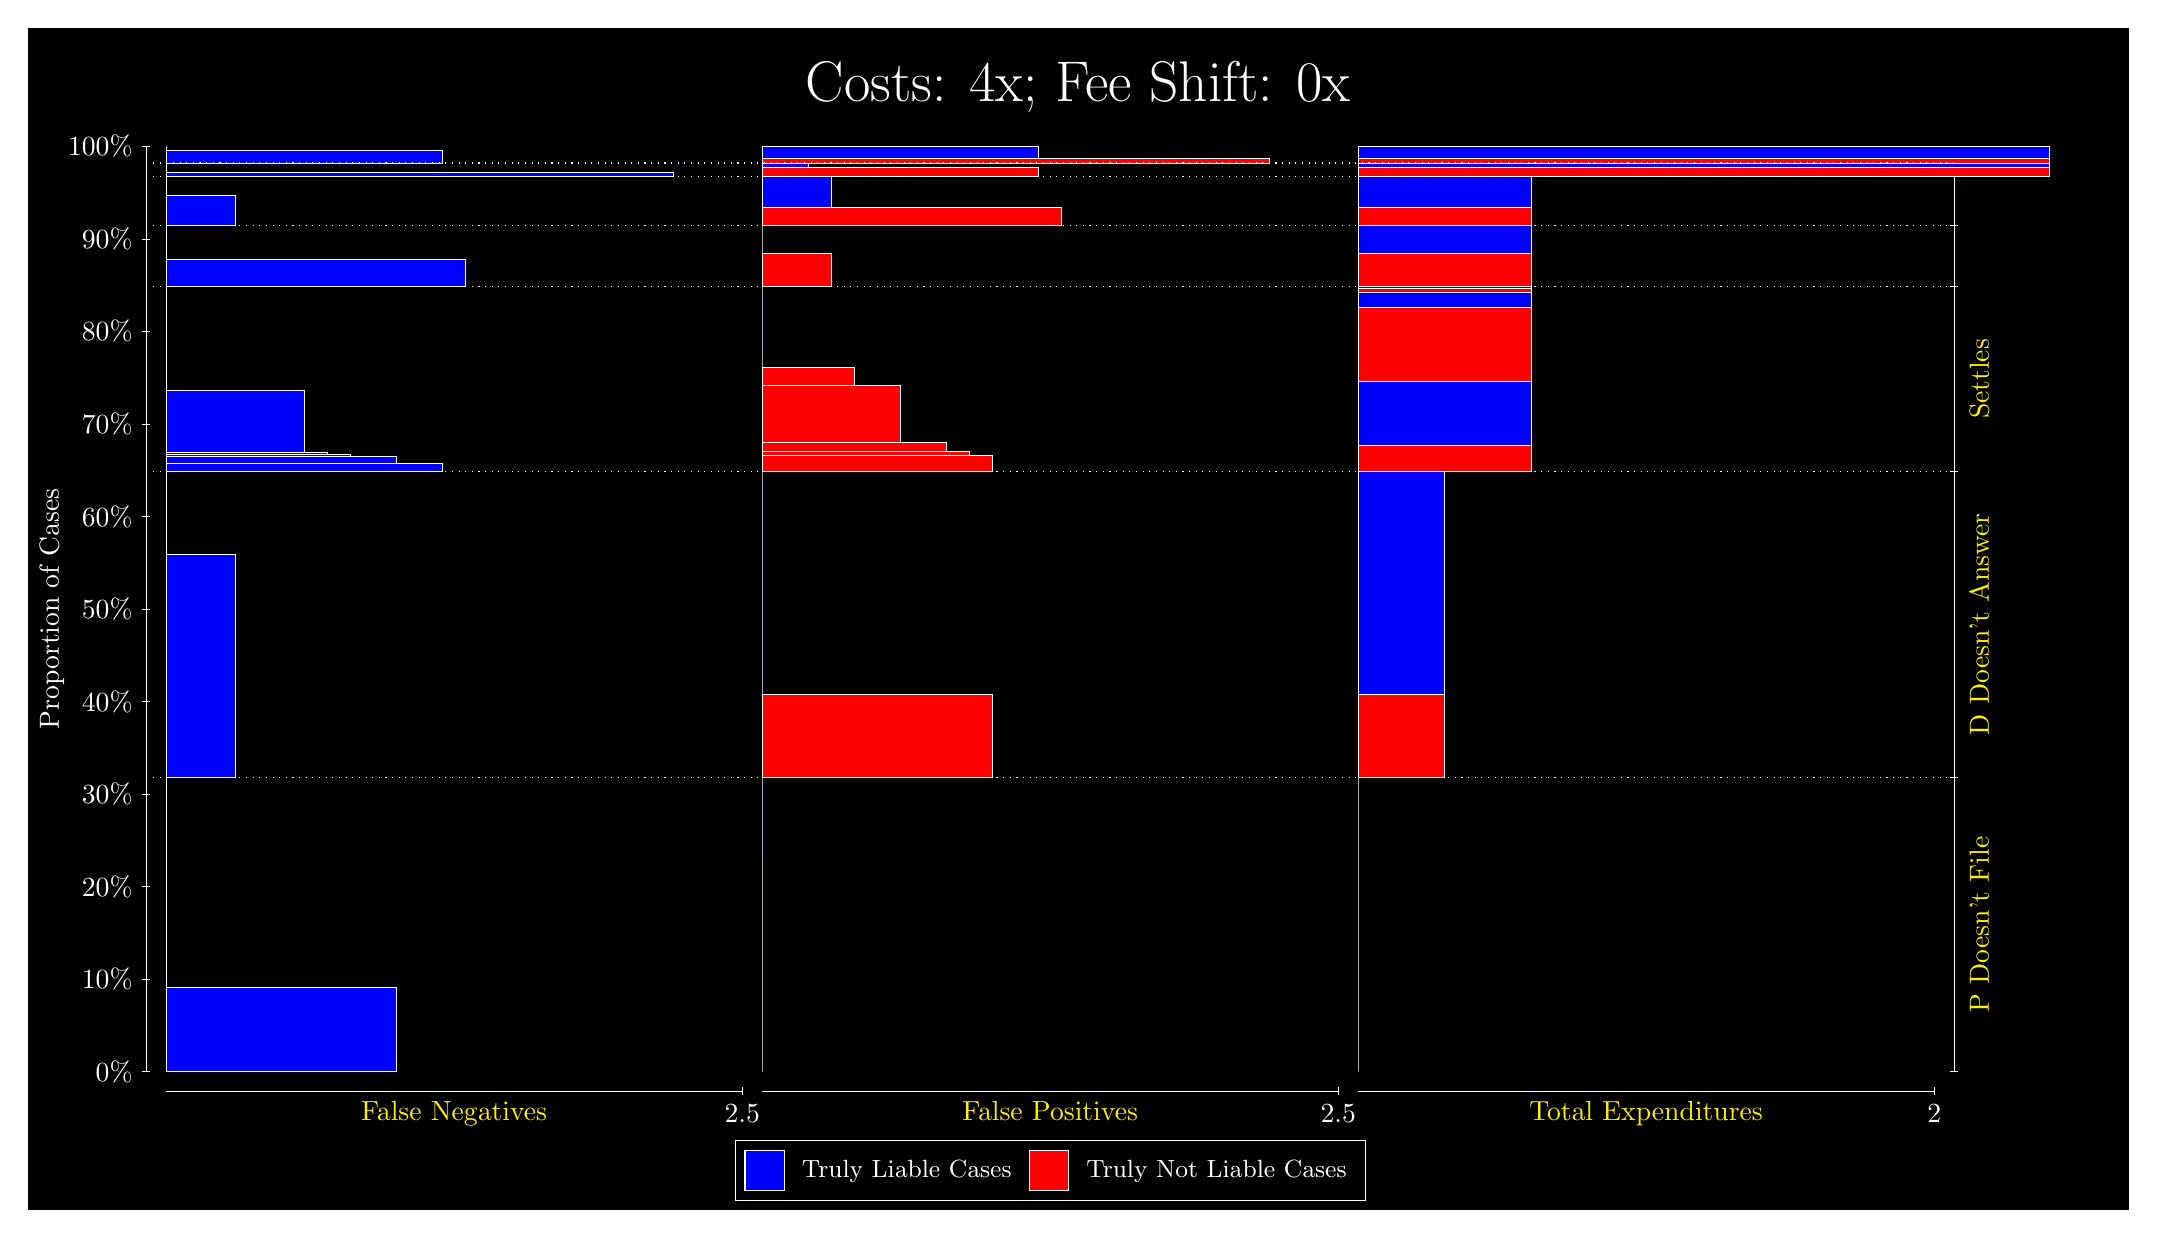
\begin{tikzpicture}
\draw[fill=black] (0,0) rectangle (26.667,15);
\draw[text=white] (0,13.5) rectangle (26.667,15) node[midway] {\huge Costs: 4x; Fee Shift: 0x};
\draw[white, very thin] (1.5,1.75) -- (1.5,13.5);
\node[rotate=90, text=white, anchor=center] at (0.3, 7.625) {Proportion of Cases};
\draw[white, very thin] (1.45,1.75) -- (1.55,1.75);
\node[text=white, anchor=east] at (1.45, 1.75) {0\%};
\draw[white, very thin] (1.45,2.925) -- (1.55,2.925);
\node[text=white, anchor=east] at (1.45, 2.925) {10\%};
\draw[white, very thin] (1.45,4.1) -- (1.55,4.1);
\node[text=white, anchor=east] at (1.45, 4.1) {20\%};
\draw[white, very thin] (1.45,5.275) -- (1.55,5.275);
\node[text=white, anchor=east] at (1.45, 5.275) {30\%};
\draw[white, very thin] (1.45,6.45) -- (1.55,6.45);
\node[text=white, anchor=east] at (1.45, 6.45) {40\%};
\draw[white, very thin] (1.45,7.625) -- (1.55,7.625);
\node[text=white, anchor=east] at (1.45, 7.625) {50\%};
\draw[white, very thin] (1.45,8.8) -- (1.55,8.8);
\node[text=white, anchor=east] at (1.45, 8.8) {60\%};
\draw[white, very thin] (1.45,9.975) -- (1.55,9.975);
\node[text=white, anchor=east] at (1.45, 9.975) {70\%};
\draw[white, very thin] (1.45,11.15) -- (1.55,11.15);
\node[text=white, anchor=east] at (1.45, 11.15) {80\%};
\draw[white, very thin] (1.45,12.325) -- (1.55,12.325);
\node[text=white, anchor=east] at (1.45, 12.325) {90\%};
\draw[white, very thin] (1.45,13.5) -- (1.55,13.5);
\node[text=white, anchor=east] at (1.45, 13.5) {100\%};

\draw[white, very thin] (24.457,1.75) -- (24.457,13.5);
\draw[white, very thin] (24.407,1.75) -- (24.507,1.75);
\node[anchor=west] at (24.407, 1.75) {};
\draw[white, very thin] (24.407,5.4875) -- (24.507,5.4875);
\node[anchor=west] at (24.407, 5.4875) {};
\draw[white, very thin] (24.407,9.375) -- (24.507,9.375);
\node[anchor=west] at (24.407, 9.375) {};
\draw[white, very thin] (24.407,11.718) -- (24.507,11.718);
\node[anchor=west] at (24.407, 11.718) {};
\draw[white, very thin] (24.407,12.494) -- (24.507,12.494);
\node[anchor=west] at (24.407, 12.494) {};
\draw[white, very thin] (24.407,13.118) -- (24.507,13.118);
\node[anchor=west] at (24.407, 13.118) {};
\draw[white, very thin] (24.407,13.288) -- (24.507,13.288);
\node[anchor=west] at (24.407, 13.288) {};
\draw[white, very thin] (24.407,13.5) -- (24.507,13.5);
\node[anchor=west] at (24.407, 13.5) {};

\draw[white, very thin, fill=blue] (1.75,1.75) rectangle (4.6775,2.8146);
\draw[white, very thin, fill=red] (1.75,2.8146) rectangle (1.75,5.4875);
\draw[white, very thin, fill=blue] (1.75,5.4875) rectangle (2.6283,8.3247);
\draw[white, very thin, fill=red] (1.75,8.3247) rectangle (1.75,9.375);
\draw[white, very thin, fill=blue] (1.75,9.375) rectangle (5.2631,9.4718);
\draw[white, very thin, fill=blue] (1.75,9.4718) rectangle (4.6775,9.5615);
\draw[white, very thin, fill=blue] (1.75,9.5615) rectangle (4.092,9.5847);
\draw[white, very thin, fill=blue] (1.75,9.5847) rectangle (3.7993,9.6116);
\draw[white, very thin, fill=blue] (1.75,9.6116) rectangle (3.5065,10.401);
\draw[white, very thin, fill=red] (1.75,10.401) rectangle (1.75,11.718);
\draw[white, very thin, fill=blue] (1.75,11.718) rectangle (5.5558,12.066);
\draw[white, very thin, fill=red] (1.75,12.066) rectangle (1.75,12.494);
\draw[white, very thin, fill=blue] (1.75,12.494) rectangle (2.6283,12.882);
\draw[white, very thin, fill=red] (1.75,12.882) rectangle (1.75,13.118);
\draw[white, very thin, fill=blue] (1.75,13.118) rectangle (8.1906,13.174);
\draw[white, very thin, fill=red] (1.75,13.174) rectangle (1.75,13.288);
\draw[white, very thin, fill=blue] (1.75,13.288) rectangle (5.2631,13.444);
\draw[white, very thin, fill=red] (1.75,13.444) rectangle (1.75,13.5);
\draw[white, very thin, fill=red] (9.3189,1.75) rectangle (9.3189,4.4229);
\draw[white, very thin, fill=blue] (9.3189,4.4229) rectangle (9.3189,5.4875);
\draw[white, very thin, fill=red] (9.3189,5.4875) rectangle (12.246,6.5378);
\draw[white, very thin, fill=blue] (9.3189,6.5378) rectangle (9.3189,9.375);
\draw[white, very thin, fill=red] (9.3189,9.375) rectangle (12.246,9.5738);
\draw[white, very thin, fill=red] (9.3189,9.5738) rectangle (11.954,9.6221);
\draw[white, very thin, fill=red] (9.3189,9.6221) rectangle (11.661,9.7467);
\draw[white, very thin, fill=red] (9.3189,9.7467) rectangle (11.075,10.461);
\draw[white, very thin, fill=red] (9.3189,10.461) rectangle (10.49,10.693);
\draw[white, very thin, fill=blue] (9.3189,10.693) rectangle (9.3189,11.718);
\draw[white, very thin, fill=red] (9.3189,11.718) rectangle (10.197,12.147);
\draw[white, very thin, fill=blue] (9.3189,12.147) rectangle (9.3189,12.494);
\draw[white, very thin, fill=red] (9.3189,12.494) rectangle (13.125,12.73);
\draw[white, very thin, fill=blue] (9.3189,12.73) rectangle (10.197,13.118);
\draw[white, very thin, fill=red] (9.3189,13.118) rectangle (12.832,13.232);
\draw[white, very thin, fill=blue] (9.3189,13.232) rectangle (9.9044,13.288);
\draw[white, very thin, fill=red] (9.3189,13.288) rectangle (15.759,13.344);
\draw[white, very thin, fill=blue] (9.3189,13.344) rectangle (12.832,13.5);
\draw[white, very thin, fill=red] (16.888,1.75) rectangle (16.888,4.4229);
\draw[white, very thin, fill=blue] (16.888,4.4229) rectangle (16.888,5.4875);
\draw[white, very thin, fill=red] (16.888,5.4875) rectangle (17.986,6.5378);
\draw[white, very thin, fill=blue] (16.888,6.5378) rectangle (17.986,9.375);
\draw[white, very thin, fill=red] (16.888,9.375) rectangle (19.083,9.6983);
\draw[white, very thin, fill=blue] (16.888,9.6983) rectangle (19.083,10.511);
\draw[white, very thin, fill=red] (16.888,10.511) rectangle (19.083,11.457);
\draw[white, very thin, fill=blue] (16.888,11.457) rectangle (19.083,11.643);
\draw[white, very thin, fill=red] (16.888,11.643) rectangle (19.083,11.692);
\draw[white, very thin, fill=blue] (16.888,11.692) rectangle (19.083,11.718);
\draw[white, very thin, fill=red] (16.888,11.718) rectangle (19.083,12.147);
\draw[white, very thin, fill=blue] (16.888,12.147) rectangle (19.083,12.494);
\draw[white, very thin, fill=red] (16.888,12.494) rectangle (19.083,12.73);
\draw[white, very thin, fill=blue] (16.888,12.73) rectangle (19.083,13.118);
\draw[white, very thin, fill=red] (16.888,13.118) rectangle (25.67,13.232);
\draw[white, very thin, fill=blue] (16.888,13.232) rectangle (25.67,13.288);
\draw[white, very thin, fill=red] (16.888,13.288) rectangle (25.67,13.344);
\draw[white, very thin, fill=blue] (16.888,13.344) rectangle (25.67,13.5);
\draw[white, dotted] (1.5,5.4875) -- (24.457,5.4875);
\draw[white, dotted] (1.5,9.375) -- (24.457,9.375);
\draw[white, dotted] (1.5,11.718) -- (24.457,11.718);
\draw[white, dotted] (1.5,12.494) -- (24.457,12.494);
\draw[white, dotted] (1.5,13.118) -- (24.457,13.118);
\draw[white, dotted] (1.5,13.288) -- (24.457,13.288);
\draw[white, very thin] (1.75,1.5) -- (9.0689,1.5);
\node[text=yellow, anchor=north] at (5.4094, 1.5) {False Negatives};
\draw[white, very thin] (9.0689,1.45) -- (9.0689,1.55);
\node[text=white, anchor=north] at (9.0689, 1.45) {2.5};

\draw[white, very thin] (9.3189,1.5) -- (16.638,1.5);
\node[text=yellow, anchor=north] at (12.978, 1.5) {False Positives};
\draw[white, very thin] (16.638,1.45) -- (16.638,1.55);
\node[text=white, anchor=north] at (16.638, 1.45) {2.5};

\draw[white, very thin] (16.888,1.5) -- (24.207,1.5);
\node[text=yellow, anchor=north] at (20.547, 1.5) {Total Expenditures};
\draw[white, very thin] (24.207,1.45) -- (24.207,1.55);
\node[text=white, anchor=north] at (24.207, 1.45) {2};

\node[text=yellow, centered, rotate=90] at (24.777, 3.6188) {P Doesn't File};
\node[text=yellow, centered, rotate=90] at (24.777, 7.4313) {D Doesn't Answer};
\node[text=yellow, centered, rotate=90] at (24.777, 10.547) {Settles};





\draw (12.978300999999998,1.5) node[draw=none] (baseCoordinate) {};
\begin{scope}[align=center]
        \matrix[scale=0.5, draw=white, below=0.5cm of baseCoordinate, nodes={draw}, column sep=0.1cm]{
            \node[rectangle, draw, minimum width=0.5cm, minimum height=0.5cm, fill=blue] {}; &
            \node[draw=none, font=\small, text=white] (B) {Truly Liable Cases}; &
            \node[rectangle, draw, minimum width=0.5cm, minimum height=0.5cm, fill=red] {}; &
            \node[draw=none, font=\small, text=white] (B) {Truly Not Liable Cases}; \\
            };
\end{scope}

\end{tikzpicture}
\end{document}